Let's say you need computational resources\ldots

Maybe you're a scientist who needs to run some simulations. You have specific hardware requirements, but you're not particularly picky about when the simulations run, and probably won't even notice if they are interrupted at some point, as long as they finish running (correctly) at some point, maybe before a given deadline. A cluster managed by a job scheduler would probably be a good fit for you.

You could also be a software developer who wants to test his or her code on a pristine machine, which you would only need for a relatively short period of time. Plus, every time you use this machine, you'd like it to start up with the exact same pristine software environment. Oh, and you want your machine now. As in \emph{right now}. One option could be to install a virtual machine (VM) manager (such as Xen, VMWare, etc.) to start up these pristine machines as VMs on your own machine. Even better, you could go to a cloud (like Amazon EC2, \url{http://www.amazon.com/ec2/}, or the Science Clouds, \url{http://workspace.globus.org/clouds/}) and have those VMs appear automagically somewhere else, so you don't have to worry about setting up the VM manager or having a machine powerful enough to run those VMs.

Or perhaps you're a run-of-the-mill geek who wants his or her own web/mail/DNS/etc server. This server will presumably be running for months or even years with high availability: your server has to be running all the time, with no interruptions. There's a whole slew of hosting providers who can give you a dedicated server or a virtual private server. The latter are typically managed with VM-based datacenter managers.

As you can see, there are a lot of resource provisioning scenarios in nature. However, the solutions that have emerged tend to be specific to a particular scenario, to the exclusion of other ones. For example, while job-based systems are exceptionally good at managing complex batch workloads, they're not too good at provisioning resources at specific times (some job-based systems do offer advance reservations, but they have well-known utilization problems) or at giving users unfettered access to provisioned resources (forcing them, instead, to interact with the resources through the job abstraction).

A lease is a general resource provisioning abstraction that could be used to satisfy a variety of use cases, such as the ones described above. In our work, we've defined a lease as a ``negotiated and renegotiable agreement between a resource provider and a resource consumer, where the former agrees to make a set of resource available to the latter, based on a set of lease terms presented by the resource consumer''. In our view, the lease terms must include the following dimensions:

\begin{description}
 \item[Hardware] The hardware resources (CPU, memory, etc.) required by the resource consumer.
 \item[Software] The software environment that must be installed in those resources.
 \item[Availability] The period during which the hardware and software resources must be available. It is important to note that the availability period can be specified in a variety of ways, like ``just get this to me as soon as you can'', ``I need this from 2pm to 4pm on Mondays, Wednesdays, and Fridays (and, if I don't get exactly this, I will be a very unhappy resource consumer)'', or even ``I need four hours sometime before 5pm tomorrow, although if you get the resources to me right now I'll settle for just two hours''. A lease-based system must be able to efficiently combine all these different types of availability.
\end{description}

Furthermore, if you don't get any of these dimensions, then you're being shortchanged by your resource lessor. For example, Amazon EC2 is very good at providing exactly the software environment you want, and reasonably good at providing the hardware you want (although you're limited to a few hardware configurations), but not so good at supporting a variety of availability periods.

So, Haizea aims to support resource leasing along these three dimension. For now, Haizea supports three types of availability:

\begin{description}
\item[Best-effort lease] Resources are provisioned as soon as they are available.
\item[Advance reservation-style leases (or "AR leases")] Resources are provisioned during a strictly defined time period (e.g., from 2pm to 4pm).
\item[Immediate leases] Resources must be provisioned right now, or not at all.
\end{description}

Although there are many systems (particularly job-based systems) that support the first two types of availability, Haizea differs in that it efficiently schedules heterogeneous workloads (combining best-effort and AR leases), overcoming the utilization problems that tend to occur when using ARs. Haizea does this by using virtual machines to implement leases. Virtual machines also enable Haizea to provide exactly the hardware and software requested by the user. Additionally, Haizea also manages the overhead of preparing a lease, to make sure that any deployment operations (such as transferring a VM disk image) are taken care of before the start of a lease, instead of being deducted from the lessee's allocation.

In the future, Haizea will support additional lease types, such as urgent leases, periodic leases, deadline-driven leases, etc.

\section{Supported types of leases}

To better illustrate the types of leases supported in Haizea, let's assume you have a 4-node cluster, and that you want to lease parts of that cluster over time. We'll represent the four nodes over time like this:

\begin{center}
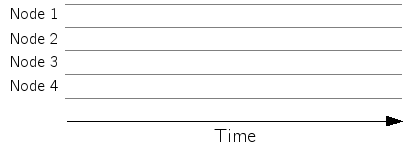
\includegraphics{images/quickstart_leasegraph1.png}
\end{center}

\subsection{``Advance Reservation'' lease}

An advance reservation, or AR, lease is a lease that must begin and end at very specific times. For example, the following lease starts at 1pm and ends at 2pm:

\begin{center}
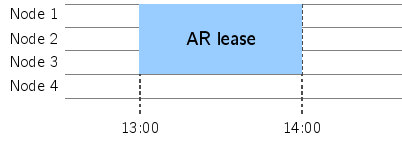
\includegraphics{images/lease_ar.png}
\end{center}

Haizea can schedule this type of lease, which is particularly useful when you need resources at a specific time (for example, to coincide with a lecture, an experiment, etc.)

\subsection{Preemptible best-effort lease}

Sometimes, you know you need resources, but you don't need them at a specific time. In fact, you're perfectly content to wait until there are enough resources available for your lease:

\begin{center}
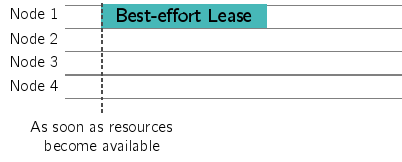
\includegraphics{images/lease_be1.png}
\end{center}


When you request a best-effort lease, your request gets placed in a queue, which is processed in a first-come-first-serve basis (the queue uses backfilling algorithms to improve resource utilization). The downside of this type of lease, of course, is that you may have to wait a while until resources are allocated to your lease:

\begin{center}
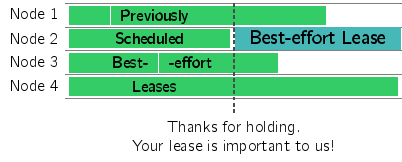
\includegraphics{images/lease_be2.png}
\end{center}

Furthermore, your lease may be running an unattended program which can be safely paused for a while (since no one is interactively using the lease resources). By requesting a preemptible lease, you allow your resources to be preempted by higher-priority leases, like advance reservations:

\begin{center}
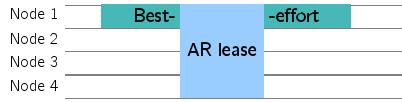
\includegraphics{images/lease_be3.png}
\end{center}

Preemptible best-effort leases are good for running batch jobs, or any non-interactive work. The Haizea paper ``Combining Batch Execution and Leasing Using Virtual Machines'' showed how using the suspend/resume capability of virtual machines allowed AR and best-effort leases to be scheduled together efficiently, overcoming the utilization problems typically associated with ARs.

\subsection{Non-preemptible best-effort lease}

But what if you're willing to wait for your resources to become available, but don't want them to be preempted? (e.g., if you want to use them interactively). Well, it's as simple as requesting a non-preemptible best-effort lease. Once your request makes it through the queue, and your lease is allocated resources, no one is taking them away.

\subsection{Immediate lease}

In some cases, you may need resources now. As in \emph{right now}:

\begin{center}
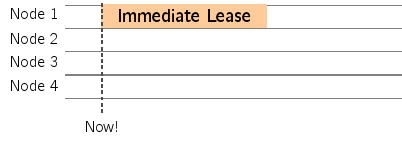
\includegraphics{images/lease_im.png}
\end{center}


Furthermore, if you can't get them right now, you're just not interested in anything else the resource provider has to offer. You're not going to request resources in the future, and you're certainly not going to be put on a queue. This is essentially the type of lease that many cloud systems offer (although the definition of "right now" varies wildly). Take into account that an immediate lease may still take a while to setup (VM image deployment, etc.). This type of lease in Haizea may evolve in the future into an ``urgent lease'', where ``right now'' really does mean ``right now''.

\subsection{Coming soon\ldots}

In the future, Haizea will support more types of leases, such as best-effort leases with deadlines and leases requiring a non-trivial negotiation before the lease is accepted.

\subsubsection{Best-effort with deadlines}

In some cases, when you say ``best effort'', you really mean ``best effort, but be reasonable''. Sure, you're willing to wait for your resources, but you may need them before a deadline.

\begin{center}
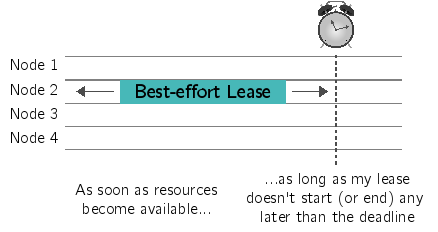
\includegraphics{images/lease_deadline.png}
\end{center}


For example, let's say you want a 16-node cluster sometime today to run a test program. You're not particularly picky about when you get the cluster, as long as it happens today and you're given sufficient warning of when your lease will be available. In the future, you will be able to tell Haizea that you have a deadline, and Haizea will either get the resources to you by then, or tell you that the deadline is simply unfeasible.

\subsubsection{Negotiated leases}

If you've ever entered into any sort of non-computational lease agreement, you know that agreeing on the lease terms rarely involves the lessor instantly being on the same page as you. Rather, it involves a fair amount of haggling. Besides, if your computational needs are flexible, so should your lease manager (c'mon, are you sure you mean "exactly at 2pm"? maybe you meant to say "at some point this afternoon"?). In the future, you will be able to negotiate your leases with Haizea:

\begin{center}
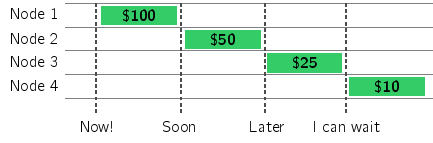
\includegraphics{images/lease_negotiate.png}
\end{center}


So, hey, maybe we can't get you that shiny AR you want at 2pm, but how about I get you twice the resources at an off-peak time? I'll even throw in a discount. And free air conditioning.